\documentclass[aspectratio=1610]{beamer}

\usetheme{KTH}
\usepackage{preamble}

\usepackage[backend=bibtex]{biblatex}

\addbibresource{references.bib}

\renewcommand{\footnotesize}{\tiny}

% Advice from Schule, that was given to him as advice when he was becoming a researcher.
%
% Three thirds, 1 third for everybody, 1 third for experts, and 1 third for yourself to show off.

% ====>>>>> general

%% The slides should be for the audience, to give them a visual experience.
%% Transitions; one style for the slides and one style for the transitions between topics. e.g. light background, dark text vs. dark background, light text.
%% Don't write too much on the slides.
%% Skip effects.
%% Masking images to direct attention.
%% Simple charts and graphs. If possible, in the same style as the presentation (e.g. fonts, colors).

\begin{document}

% Add page numbers.
\addtobeamertemplate{navigation symbols}{}{\insertframenumber / \inserttotalframenumber}

% === [ Start page ] ===========================================================

\startpage

\begin{frame}
	\vspace{0.02\textheight}

	\begin{Large}
		``Fuzzy morphisms between graphs'' {\small (Perchant \& Bloch, 2002)} and \\ ``Fuzzy graphs'' {\small (Rosenfeld, 1975)}
	\end{Large}

	\vspace{0.1\textheight}

	\begin{small}
		\textit{Robin Eklind}
	\end{small}
\end{frame}

% === [ Disposition ] ==========================================================

\normalpage

\begin{frame}
	\frametitle{Disposition}

	\begin{enumerate}
		\item Primer \textit{Fuzzy Graph Theory}
		\item What? \textit{Fuzzy Graph Isomorphisms}
		\item Why? \textit{Applications of Fuzzy Graph Isomorphisms}
		\item How? \textit{Locating Fuzzy Graph Isomorphisms}
		\item Conclusions
		\item Demo!
	\end{enumerate}
\end{frame}


% === [ Introduction ] =========================================================

% ====>>>>> Primer

% Fuzzy Graph Theory

% Quickly cover the background terminology of Fuzzy Logic and Fuzzy Graph
% Theory.

\begin{frame}
	\frametitle{A Primer to Fuzzy Graph Theory}

	% Fuzzy Logic used to handle uncertainty.
	\todo{remove this subdisposition?}
	\begin{enumerate}
		\item Fuzzy Logic
		\item Fuzzy Graph Theory
	\end{enumerate}
\end{frame}

\begin{frame}
	\frametitle{Fuzzy Logic}

	\begin{block}{Fuzzy Subsets}
		% sigma
		A \textit{fuzzy subset} of a set $S$ is a mapping $\sigma: S \rightarrow [0, 1]$ which assigns each item $x \in S$ a degree of membership $0 \le \sigma(x) \le 1$.

		\vspace*{2em}

		Examples:
		\begin{itemize}
			\item $Deina \in old$ with $\sigma(Deina) = 0.3$
			\begin{itemize}
				\item The item $Deina$ (woman at age $34$) is a member of the set $old$ to a degree of $0.3$
			\end{itemize}
			\item $Foufoutos \in old$ with $\sigma(Foufoutos) = 0.5$
			\begin{itemize}
				\item The item $Foufoutos$ (man at age $45$) is a member of the set $old$ to a degree of $0.5$
			\end{itemize}
			\item $Tade \in old$ with $\sigma(Tade) = 0.1$
			\begin{itemize}
				\item The item $Tade$ (boy at age $6$) is a member of the set $old$ to a degree of $0.1$
			\end{itemize}
		\end{itemize}
	\end{block}
\end{frame}


% contributions:
% * show how to generalize fuzzy relationship to map into a fuzzy subset of a set $S$.
% * present fuzzy analogs of graph-theoretic concepts.

\begin{frame}
	\frametitle{Fuzzy Logic}

	\begin{block}{Fuzzy Relationships}
		% mu
		A \textit{fuzzy relationship} on a set $S$ is a mapping $\mu: S \times S \rightarrow [0, 1]$ which assigns each ordered pair $(x, y) \in S \times S$ a degree of membership $0 \le \mu(x, y) \le 1$. In other words, a fuzzy relatipship on $S$ is a fuzzy subset of $S \times S$.

		\vspace*{2em}

		Examples:
		\begin{itemize}
			\item $(Deina, Tade) \in mothers$ with $\mu(Deina, Tade) = 1.0$, where $mothers: person \times person$
			\begin{itemize}
				\item The ordered pair $(Deina, Tade)$ is a $(mother, child)$-relationship on the set $person$ to a degree of $1.0$
			\end{itemize}
			\item $(Foufoutos, Tade) \in fathers$ with $\mu(Foufoutos, Tade) = 0.5$, where $fathers: person \times person$
			\begin{itemize}
				\item The ordered pair $(Foufoutos, Tade)$ is a $(father, child)$-relationship on the set $person$ to a degree of $0.5$
			\end{itemize}
		\end{itemize}
	\end{block}
\end{frame}

\begin{frame}
	\frametitle{Fuzzy Graph Theory}

	\begin{block}{Fuzzy Logic Analogies in Graph Theory}
		\todo{find proper name for $F(\sigma, \mu)$}

		Given a graph $G(V, E)$ with verticies $v \in V$ and edges $e \in E$, a fuzzy graph $F(\sigma, \mu)$ represent verticies as a \textit{fuzzy subset} $\sigma: V \rightarrow [0, 1]$ of $V$ and the edges as a \textit{fuzzy relatipship} $\mu: V \times V \rightarrow [0, 1]$ on $V$. In other words, since $E: V \times V$, $\mu: E \rightarrow [0, 1]$.
	\end{block}
\end{frame}

% ====>>>>> What?

% What?

% Frame problem at a high level.
% 1-3 minutes.

% Key message you wish to communicate. From the perspective of the audience, what will they gain? What can they do with the information?

\begin{frame}
	\frametitle{What?}

	(Sub)graph isomorphism requires a \textit{bijective} mapping to match verticies and edges of two graphs. In other words, there may exist no missing or additional verticies or edges.

	\vspace*{2em}

	The real world is not ideal, as such we are often interested in \textit{inexact} graph matches.

	\vspace*{2em}

	\textit{Fuzzy graph morphisms} are used to formalize inexact graph matches.
\end{frame}

\begin{frame}
	\frametitle{Fuzzy Graph Morphisms}

	\begin{block}{Fuzzy Graph Morphisms}
		\textbf{Definition}: A \textit{fuzzy morphism} $(\rho_{\sigma}, \rho_{\mu})$ between graphs $G_1$ and $G_2$ is a pair of mappings $\rho_{\sigma}: N_1 \times N_2 \rightarrow [0, 1]$ and $\rho_{\mu}: N_1 \times N_2 \times N_1 \times N_2 \rightarrow [0, 1]$ which satisfy:

		\begin{equation}
			\begin{aligned}
				& \forall (u_1, v_1) \in N_1 \times N_1, \forall (u_2, v_2) \in N_2 \times N_2: \\
				& \rho_{\mu}(u_1, u_2, v_1, v_2) \le \rho_{\sigma}(u_1, u_2) \fuzzmin \rho_{\sigma}(v_1, v_2)
			\end{aligned}
			\label{eq:fuzzy_morphism_relation}
		\end{equation}

		\textbf{Corollary}: A fuzzy morphism $(\rho_{\sigma}, \rho_{\mu})$ is a fuzzy graph, and equation \ref{eq:fuzzy_morphism_relation} is analogous to equation \ref{eq:fuzzy_relation}.

		\vspace*{2em}

		The mapping $\rho_{\sigma}$ is called a \textit{vertex morphism} and $\rho_{\mu}$ a \textit{edge morphism}.
	\end{block}
\end{frame}

\begin{frame}
	\frametitle{Fuzzy Graph Morphisms}

	\textbf{Example}:
	\begin{figure}[htbp]
		\centering
		\begin{subfigure}[t]{0.26\textwidth}
			\centering
			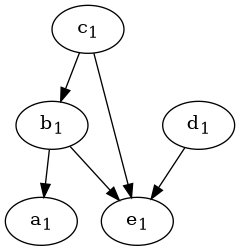
\includegraphics[width=\linewidth,valign=t]{inc/fuzzy_graph_theory/fuzzy_graph_morphism_G1.png}
			\caption{$G_1$.}
		\end{subfigure}
		\quad
		\begin{subfigure}[t]{0.19\textwidth}
			\centering
			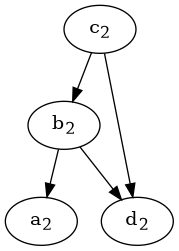
\includegraphics[width=\linewidth,valign=t]{inc/fuzzy_graph_theory/fuzzy_graph_morphism_G2.png}
			\caption{$G_2$.}
		\end{subfigure}
		\caption{Example graphs $G_1$ (left) and $G_2$ (right).}
	\end{figure}
\end{frame}

\begin{frame}
	\frametitle{Interal Representation of Fuzzy Graph Morphisms}

	\begin{figure}[htbp]
		\centering
		\begin{subfigure}[t]{0.20\textwidth}
			\centering
			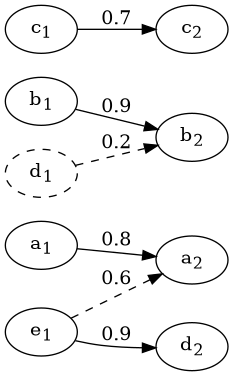
\includegraphics[width=\linewidth,valign=t]{inc/fuzzy_graph_theory/fuzzy_graph_morphism_internal_rho_sigma.png}
			\caption{Vertex morphism $\rho_{\sigma}$.}
		\end{subfigure}
		\quad
		\begin{subfigure}[t]{0.40\textwidth}
			\centering
			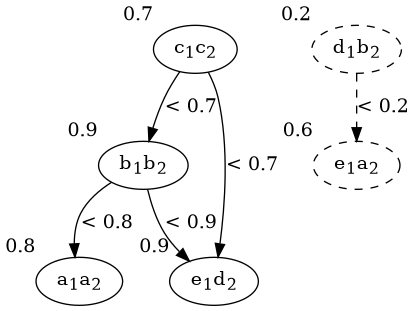
\includegraphics[width=\linewidth,valign=t]{inc/fuzzy_graph_theory/fuzzy_graph_morphism_internal_rho_mu.png}
			\caption{Edge morphism $\rho_{\mu}$.}
		\end{subfigure}
		\quad
		\begin{subfigure}[t]{0.18\textwidth}
			\begin{subfigure}[t]{\textwidth}
				\centering
				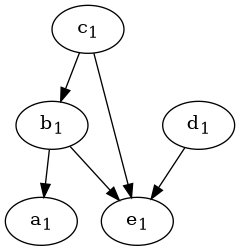
\includegraphics[width=\linewidth,valign=t]{inc/fuzzy_graph_theory/fuzzy_graph_morphism_G1.png}
				\caption{$G_1$.}
			\end{subfigure}
			\begin{subfigure}[t]{0.8\textwidth}
				\centering
				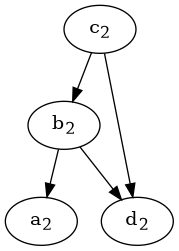
\includegraphics[width=\linewidth,valign=t]{inc/fuzzy_graph_theory/fuzzy_graph_morphism_G2.png}
				\caption{$G_2$.}
			\end{subfigure}
		\end{subfigure}
		\caption{Interal representation of fuzzy graph morphism $\rho(\sigma, \mu)$.}
	\end{figure}

\end{frame}

% ====>>>>> Why?

% Why?

% Then go into depth; both intellectual and emotional arguments for the severity of the problem.
% 15-20 minutes if presenting for 1 hour.

\begin{frame}
	\frametitle{Why?}

	\begin{block}{Applications of Fuzzy Graph Morphisms}
		\begin{itemize}
			\item Binary analysis
			\begin{itemize}
				\item Function identification by matching fuzzy graph morphisms of callgraphs, control flow and data flow graphs
			\end{itemize}
			\item Pattern recognition
			\item Image analysis
			\begin{itemize}
				\item Fuzzy graph morphisms of regions (vertices) and relation between regions (edges)
			\end{itemize}
			\item Recognition of brain structures
			\begin{itemize}
				\item Fuzzy graph morphisms of neurons (vertices) and synapses (edges)
			\end{itemize}
		\end{itemize}
	\end{block}
\end{frame}

% ====>>>>> How?

% How?

% Give solution, including benefits and drawbacks.

\begin{frame}
	\frametitle{How?}

	\begin{block}{Locating Fuzzy Graph Isomorphisms}
		\begin{itemize}
			\item General idea of how to locate fuzzy graph isomorphisms
			\item Method used in ``Fuzzy morphisms between graphs''
		\end{itemize}
	\end{block}
\end{frame}

% --- [ General idea ] ---------------------------------------------------------

\begin{frame}
	\frametitle{General idea of how to locate fuzzy graph isomorphisms}

	\todo{add general idea}

\end{frame}

\begin{frame}
	\frametitle{Method used in ``Fuzzy morphisms between graphs''}

	\todo{add illustrations}
\end{frame}

% ___ [ Fuzzy morphism - Example ] _____________________________________________

% One example for each method to illustrate how it works.

\begin{frame}
	\frametitle{Fuzzy morphism - example}
	\todo{update wording}
	Example of fuzzy morphism between the CFGs of two binary functions.

	\todo{add illustrations}
\end{frame}

\begin{frame}[noframenumbering]
	\frametitle{Fuzzy morphism - example}
	\todo{update wording}
	Example of fuzzy morphism between the CFGs of two binary functions.

	\todo{add illustrations}
\end{frame}

% === [ Conclusions ] ==========================================================

\begin{frame}
	\frametitle{Conclusions}

	\begin{enumerate}
		\item Significance of papers
		\item Relation to other research
	\end{enumerate}
\end{frame}

% --- [ Significance of papers ] -----------------------------------------------

\begin{frame}
	\frametitle{Significance of papers}

	Rosenfeld was among the first to formalized fuzzy graph theory in the seminal paper ``Fuzzy graphs'' (1975), which has since received 910 citations (and is also cited in ``Fuzzy morphisms between graphs'').

	\vspace*{2em}

	Perchant and Bloch established a formalism for inexact graph matchings in ``Fuzzy morphisms between graphs''. The paper remains less influential with 61 citations.
\end{frame}

% --- [ Relation to other research ] -------------------------------------------

% how the research relates to the larger picture, what is your personal
% view of the significance of the research. related research, both prior
% and later.

\begin{frame}
	\frametitle{Relation to other research}

% 2019-
%
% TODO: Summary of what happens in the academic community, main reserach happening.

	\begin{block}{Prior-art}
		Rosenfeld was a leading researcher of image analysis and essentially established the field; among others writing the first textbook on the topic (``Picture Processing by Computer'' in 1969, later followed by ``Digital picture processing'' in 1976, a book with 8547 citations).

		\vspace*{2em}

		Similarly, Perchant and Bloch have a background in image analysis.
	\end{block}

	\begin{block}{Follow-up research}
		Bloch went on to applied research related to cognitive science and have among others co-authored the paper ``Diffeomorphic demons: Efficient non-parametric image registration'', which has received 1106 citations to date.

		\vspace*{2em}

		In general, follow-up research seem to be more oriented towards application rather than theory.
	\end{block}
\end{frame}

\begin{frame}
	\frametitle{Demo}

Time for a demo!

\end{frame}

\begin{frame}
	\frametitle{Function identification through fuzzy callgraph matching}

\textbf{Example}: source program compiled for three different machine architectures.

	\begin{figure}[htbp]
		\centering
		\begin{subfigure}[t]{0.32\textwidth}
			\centering
			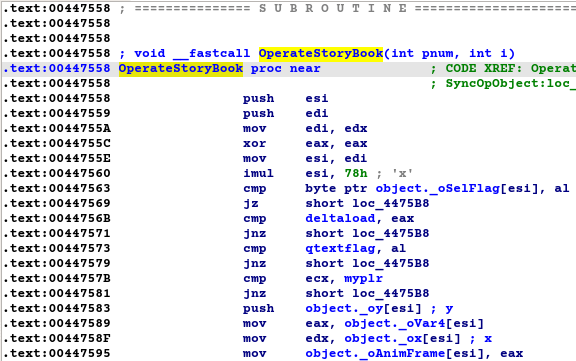
\includegraphics[width=\linewidth,valign=t]{inc/example/x86_zoom.png}
			\caption{x86 assembly.}
		\end{subfigure}
		\hfill
		\begin{subfigure}[t]{0.32\textwidth}
			\centering
			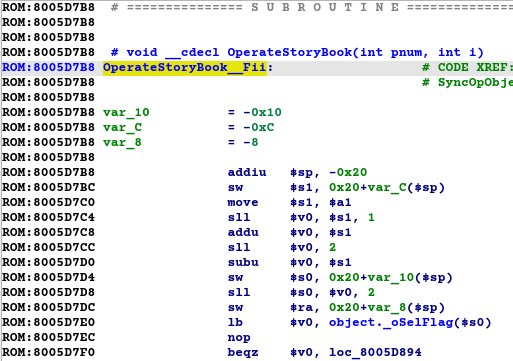
\includegraphics[width=\linewidth,valign=t]{inc/example/mips_zoom.png}
			\caption{MIPS assembly.}
		\end{subfigure}
		\hfill
		\begin{subfigure}[t]{0.32\textwidth}
			\centering
			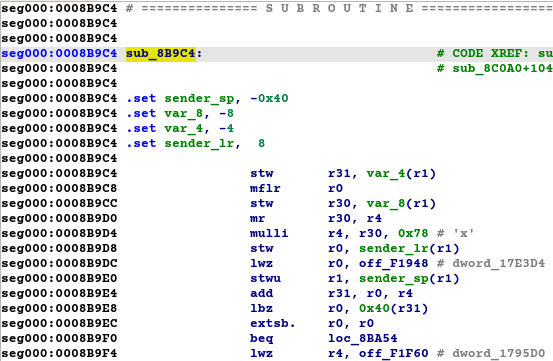
\includegraphics[width=\linewidth,valign=t]{inc/example/ppc_zoom.png}
			\caption{PowerPC assembly.}
		\end{subfigure}
		\caption{Machine code of the same source function in x86 (left), MIPS (middle) and PowerPC (right) assembly.}
	\end{figure}

\end{frame}

\begin{frame}
	\frametitle{Function identification through fuzzy callgraph matching}

	\begin{figure}[htbp]
		%\centering
		\begin{subfigure}{1\textwidth}
			\centering
			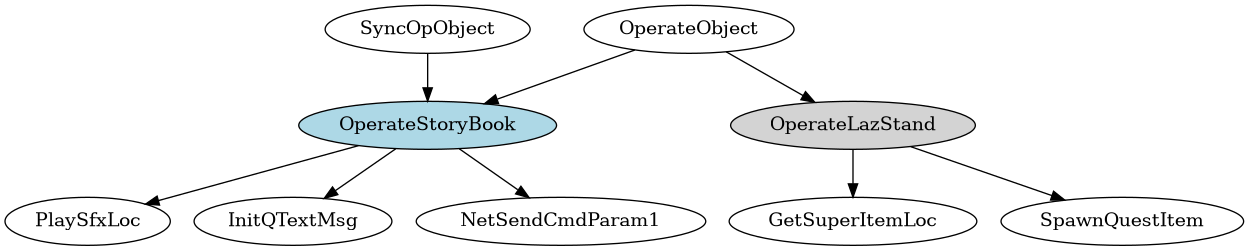
\includegraphics[width=0.65\linewidth]{inc/example/callgraph_x86.png}
			\caption{x86 callgraph.}
		\end{subfigure}
		\begin{subfigure}{1\textwidth}
			\centering
			\vspace*{1em}
			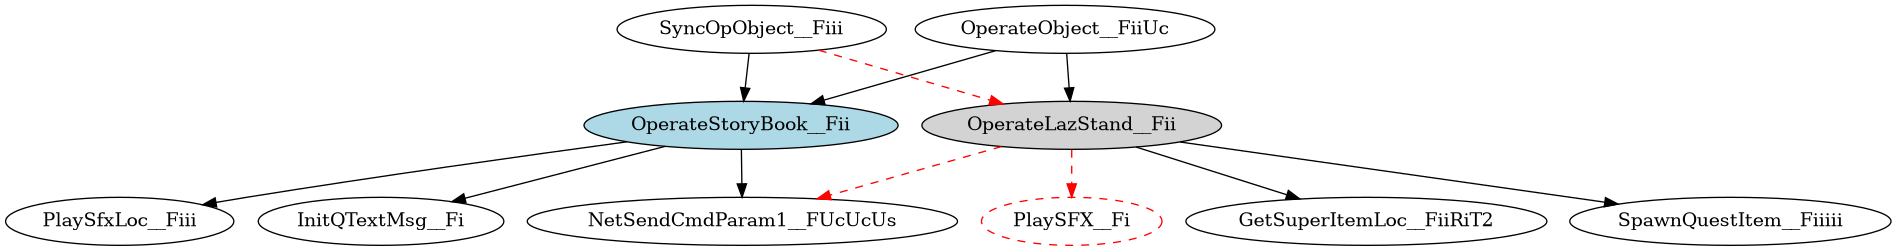
\includegraphics[width=0.9\linewidth]{inc/example/callgraph_mips.png}
			\caption{MIPS callgraph.}
		\end{subfigure}
		\begin{subfigure}{1\textwidth}
			\centering
			\vspace*{1em}
			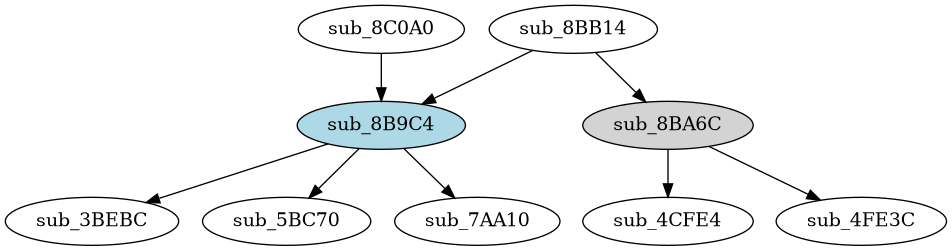
\includegraphics[width=0.5\linewidth]{inc/example/callgraph_ppc_before.png}
			\caption{PowerPC callgraph.}
		\end{subfigure}
		\caption{Corresponding callgraphs for x86 (top), MIPS (middle) and PowerPC (bottom) assembly.}
	\end{figure}

\end{frame}

\begin{frame}
	\frametitle{Function identification through fuzzy callgraph matching}

	\begin{figure}[htbp]
		%\centering
		\begin{subfigure}{1\textwidth}
			\centering
			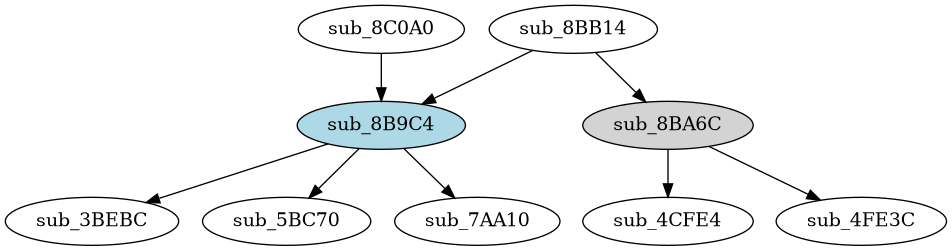
\includegraphics[width=0.7\linewidth]{inc/example/callgraph_ppc_before.png}
			\caption{MIPS callgraph \textit{before} fuzzy callgraph matching.}
		\end{subfigure}
		\begin{subfigure}{1\textwidth}
			\centering
			\vspace*{1em}
			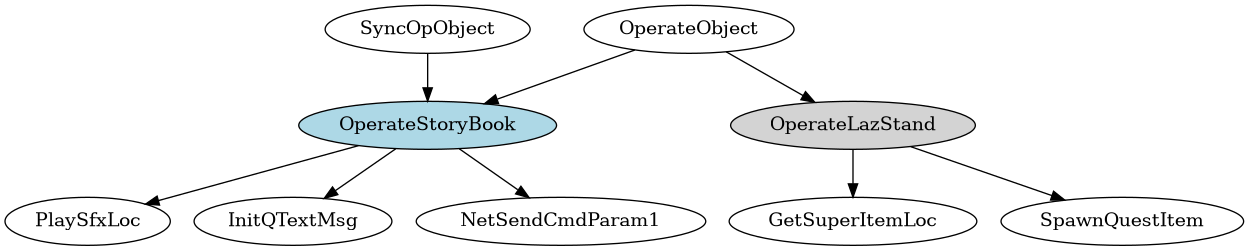
\includegraphics[width=0.9\linewidth]{inc/example/callgraph_ppc_after.png}
			\caption{MIPS callgraph \textit{after} fuzzy callgraph matching.}
		\end{subfigure}
		\caption{Results of fuzzy callgraph matching used to assign names to unknown functions.}
	\end{figure}

\end{frame}

\begin{frame}
	\frametitle{Function identification through fuzzy callgraph matching}

	The example source program has a callgraph with $2551$ verticies and $6400$ edges, illustrating the need for performant algorithms and the benefit of automating function identification.

	\begin{figure}[htbp]
		\centering
		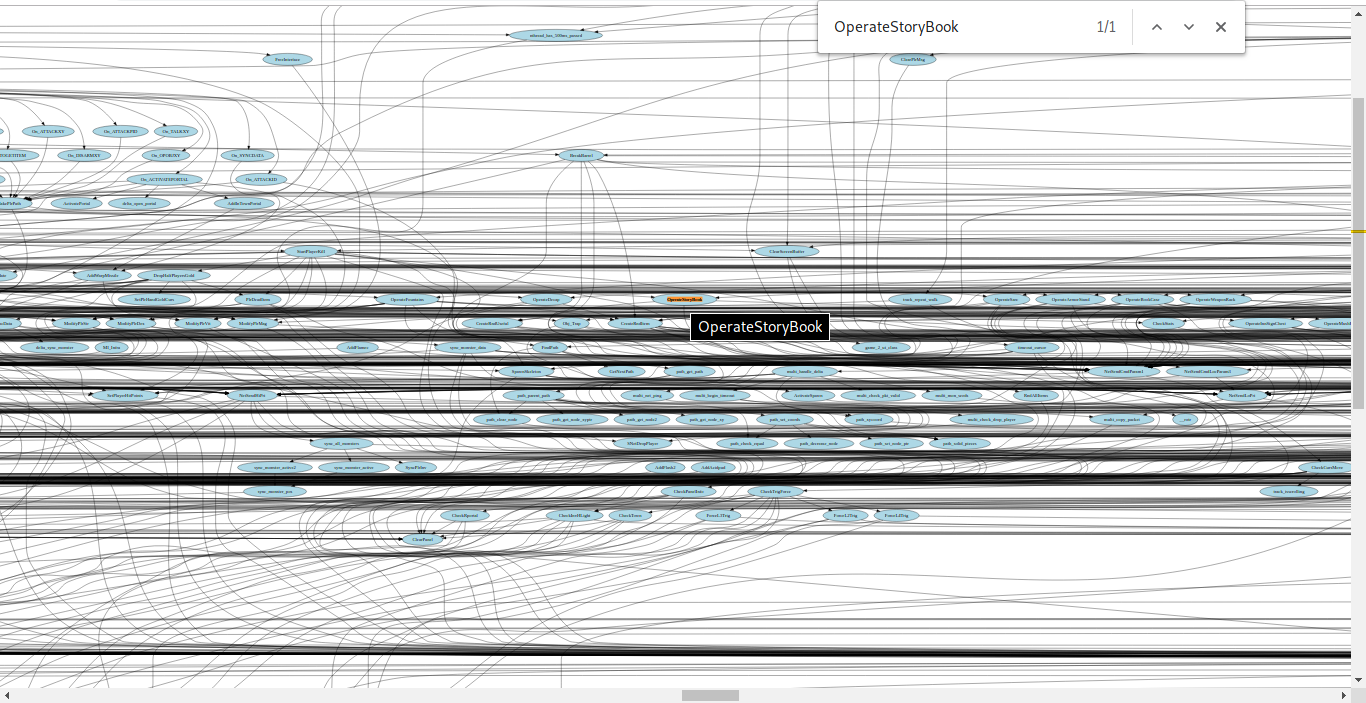
\includegraphics[width=0.85\linewidth]{inc/example/full_callgraph.png}
		\caption{An extract of the callgraph of the source program.}
	\end{figure}
\end{frame}

\begin{frame}
	\frametitle{Function identification through fuzzy callgraph matching}

	For reference, this is the original source code of the C source function \texttt{OperateStoryBook}.

	\begin{figure}[htbp]
		\centering
		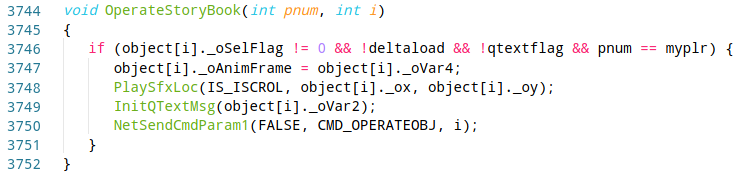
\includegraphics[width=0.8\linewidth]{inc/example/source_func_light.png}
		%\lstinputlisting[language=C, style=c]{inc/example/source_func.c}
		\caption{Original source code of the C source function \texttt{OperateStoryBook}.}
	\end{figure}
\end{frame}


\end{document}
